\documentclass[conference]{IEEEtran}
\IEEEoverridecommandlockouts
\usepackage{cite}
\usepackage{amsmath,amssymb}
\usepackage{graphicx}
\usepackage{booktabs}
\usepackage{xcolor}
\usepackage{tikz}
\usetikzlibrary{arrows.meta,positioning,fit,calc,shapes.misc,backgrounds}
\usepackage{pgfplots}
\pgfplotsset{compat=1.17}
\usepackage[hidelinks]{hyperref}
\newcommand{\sgVocab}{191}
\newcommand{\sgPairs}{1878}
\newcommand{\sgSent}{107}
\newcommand{\sgEpochs}{300}
\newcommand{\sgPearsonMin}{0.977}
\newcommand{\sgPearsonMax}{0.984}
\newcommand{\sgSameMin}{-0.28}
\newcommand{\sgSameMax}{0.09}
\newcommand{\sgWordList}{boy,cat,dog,elephant,girl,he,his,king,kitten,man,prince,puppy,queen,tiger,woman}
\newcommand{\blockParamsSmall}{12{,}704}
\newcommand{\xorSingleStart}{0.2845}
\newcommand{\xorSingleEnd}{0.2842}


% Status encoding that survives greyscale printing: solid = measured,
% dashed = in progress, dotted = designed only (not built, not measured).
\tikzset{
  box/.style={draw,rounded corners=1pt,align=center,font=\footnotesize,inner sep=3pt,minimum height=0.9cm},
  measured/.style={box,thick},
  wip/.style={box,dashed,thick},
  design/.style={box,dotted,thick},
  arr/.style={-{Stealth[length=4pt]},thick},
  small/.style={font=\scriptsize,align=center},
}

\begin{document}

\title{Rebuilding a Small Transformer from Scratch:\\
Measured Foundations and a Neuro-Symbolic Design for the Reasoning Gap\\
\large A Progress Report}

\author{\IEEEauthorblockN{Ned Pham}
\IEEEauthorblockA{School of Computer Science, University of Nottingham, UK}}

\maketitle

\begin{abstract}
We rebuild, without machine-learning libraries, the chain of ideas that leads to a GPT-style language model: a rule-based chatbot, a subword tokenizer, a network trained by back-propagation, word embeddings, and a decoder-only transformer. This paper reports what is finished and measured, and what is not. Stages 0--3 run and are tested; we report XOR learning and Skip-gram embeddings over four random seeds. The seeds reach the same function with very different weights: Skip-gram vectors for the same word differ across seeds (cosine between~$\sgSameMin$ and~$\sgSameMax$) while the pairwise geometry agrees (Pearson $r=\sgPearsonMin$--$\sgPearsonMax$). A cross-entropy objective rewards such fits but contains no term for why an output is right. We use the taxonomy of Sheth, Roy and Gaur to propose a feasible neuro-symbolic extension: a logit-level knowledge constraint and a decoupled verifier with a reasoning trace. The transformer and the symbolic layer are \emph{not yet implemented}, so we report no results for them; their experiments are specified as falsifiable predictions. Every number in this paper is regenerated by one command.
\end{abstract}

\begin{IEEEkeywords}
transformer, self-attention, neuro-symbolic AI, word embeddings, reproducibility, reasoning
\end{IEEEkeywords}

%% ------------------------------------------------------------------------
\section{Introduction}
Large language models predict the next token. A study note that motivates this work puts the consequence bluntly: the model ``guess[es] the best weight to achieve target error'' but lacks critical reasoning about its own output, its behaviour is ``pure emergent'' rather than ``designed'', and neuro-symbolic AI is named as the route out of the black box~\cite{note}. We take that statement as a hypothesis and ask two questions. (i)~What does fitting random weights to a loss actually produce in a model small enough to inspect? (ii)~What is the smallest neuro-symbolic extension that could be built and tested on such a model?

\textbf{Contributions.} (1)~A working, seeded, tested from-scratch pipeline for stages 0--3, including the diagnosis and repair of a collapsed Skip-gram implementation (Sec.~\ref{sec:measured}). (2)~A measurement of seed sensitivity: same function, different weights (Sec.~\ref{sec:measured}). (3)~A transformer specification that follows the note's order and adds the equations the note omits (Sec.~\ref{sec:transformer}). (4)~A scoped neuro-symbolic design mapped onto the taxonomy of~\cite{sheth2023}, with falsifiable predictions and stated limits (Sec.~\ref{sec:ns}).

\textbf{What this paper does not contain.} It contains no trained-transformer metric, no attention visualisation, and no symbolic-layer result, because those components do not exist yet. Figures~\ref{fig:pipeline}--\ref{fig:arch} are schematics and are labelled as such.

%% ------------------------------------------------------------------------
\section{Background and Related Work}
\emph{Transformer.} Vaswani et al.~\cite{vaswani2017} replace recurrence with scaled dot-product attention. We follow the pre-layer-norm decoder-only variant~\cite{ba2016}, trained with Adam~\cite{kingma2015}. \emph{Earlier stages.} ELIZA~\cite{weizenbaum1966} is the rule-based baseline; byte-pair encoding~\cite{sennrich2016} gives the subword vocabulary; back-propagation~\cite{rumelhart1986} trains the XOR network; Skip-gram with negative sampling~\cite{mikolov2013a,mikolov2013b} gives static embeddings.

\emph{Neuro-symbolic AI.} Sheth, Roy and Gaur~\cite{sheth2023} divide methods into \emph{lowering} (Category~1: compress symbolic knowledge for use inside a neural network) and \emph{lifting} (Category~2: lift neural patterns into symbolic form). Each splits in two, giving four subcategories (Fig.~\ref{fig:taxonomy}). The paper does not use Kautz's six patterns and does not use the terms ``learning for reasoning'' or ``reasoning for learning''; we do not either.

\emph{Reference design.} Our architecture cross-checks against a public tutorial repository~\cite{howllms}. It has no licence file, so we copied no code, and it contains no symbolic component.

%% ------------------------------------------------------------------------
\section{System and Reproducibility Protocol}
Fig.~\ref{fig:pipeline} shows the pipeline and the status of each stage. The stack is TypeScript on Bun with no ML libraries. All randomness goes through one seeded generator (Mulberry32), so a run is a pure function of its seed.

\begin{figure*}[t]
\centering
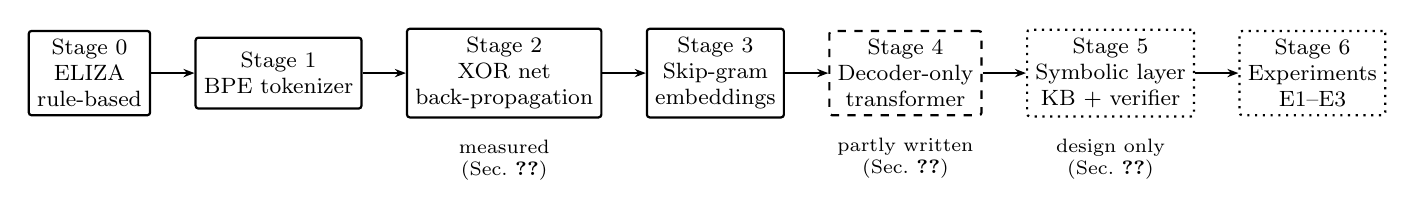
\begin{tikzpicture}[node distance=0.55cm]
  \node[measured] (e) {Stage 0\\ELIZA\\rule-based};
  \node[measured,right=of e] (b) {Stage 1\\BPE tokenizer};
  \node[measured,right=of b] (x) {Stage 2\\XOR net\\back-propagation};
  \node[measured,right=of x] (s) {Stage 3\\Skip-gram\\embeddings};
  \node[wip,right=of s] (t) {Stage 4\\Decoder-only\\transformer};
  \node[design,right=of t] (n) {Stage 5\\Symbolic layer\\KB + verifier};
  \node[design,right=of n] (ex) {Stage 6\\Experiments\\E1--E3};
  \foreach \a/\b in {e/b,b/x,x/s,s/t,t/n,n/ex} \draw[arr] (\a) -- (\b);
  \node[small,below=0.15cm of x] {measured\\(Sec.~\ref{sec:measured})};
  \node[small,below=0.15cm of t] {partly written\\(Sec.~\ref{sec:transformer})};
  \node[small,below=0.15cm of n] {design only\\(Sec.~\ref{sec:ns})};
\end{tikzpicture}
\caption{Pipeline and status. Solid border: implemented and measured. Dashed: in progress. Dotted: specified, not built. Stage 0--1 are exercised by the application but contribute no metric to this paper.}
\label{fig:pipeline}
\end{figure*}

\textbf{Reproduction.} \texttt{bun tests/ieee-data.ts} regenerates every CSV, JSON and LaTeX fragment in \texttt{docs/progress/ieee/data/}; \texttt{main.tex} reads only those files. \texttt{bun test tests/train-embed.test.ts} runs the Skip-gram sanity tests. Seeds are $\{42,1,2,3\}$. A second run of the same seed returned an identical final loss for the XOR network.

%% ------------------------------------------------------------------------
\section{Measured Results, Stages 2--3}\label{sec:measured}

\subsection{XOR: same function, different weights}
A single-layer perceptron cannot represent XOR; a $2\!\to\!4\!\to\!1$ sigmoid network trained by back-propagation can~\cite{rumelhart1986}. Loss is mean-squared error over the four inputs, learning rate~1.0, full-batch.

\begin{table*}[t]
\caption{XOR, $2\!\to\!4\!\to\!1$ network, four seeds. Outputs are for inputs $(0,0),(0,1),(1,0),(1,1)$ after 5000 epochs; the last column is the first row of the input-to-hidden weights after 5000 epochs.}
\label{tab:xor}
\centering\footnotesize
\setlength{\tabcolsep}{3pt}
\begin{tabular}{@{}lccll@{}}
\toprule
Seed & MSE@500 & MSE@5000 & Outputs & $w_1[0,:]$ \\
\midrule
42 & 0.0144 & $2.8\mathrm{e}{-4}$ & 0.01 / 0.98 / 0.98 / 0.02 & $[5.8,\,-1.5,\,6.2,\,-0.3]$ \\
1 & 0.0227 & $2.7\mathrm{e}{-4}$ & 0.01 / 0.98 / 0.98 / 0.02 & $[0.0,\,-6.5,\,-1.9,\,5.3]$ \\
2 & 0.1506 & $3.1\mathrm{e}{-4}$ & 0.01 / 0.98 / 0.98 / 0.02 & $[3.5,\,-2.6,\,-6.7,\,-5.2]$ \\
3 & 0.0110 & $2.2\mathrm{e}{-4}$ & 0.01 / 0.98 / 0.99 / 0.01 & $[4.0,\,-2.9,\,1.2,\,-6.6]$ \\
single-layer (42) & 0.2842 & -- & 0.53 / 0.50 / 0.47 / 0.43 & --
\\
\bottomrule
\end{tabular}
\end{table*}

\begin{figure}[t]
\centering
\begin{tikzpicture}
\begin{semilogyaxis}[width=\columnwidth,height=5.2cm,xlabel={epoch},ylabel={MSE},legend style={font=\scriptsize,at={(0.98,0.55)},anchor=east},tick label style={font=\scriptsize},label style={font=\footnotesize},ymin=1e-4,ymax=0.5,grid=both,grid style={gray!25}]
\addplot[thick,solid] table[x=epoch,y=seed42,col sep=comma]{data/xor_multi_loss.csv};\addlegendentry{seed 42}
\addplot[thick,dashed] table[x=epoch,y=seed1,col sep=comma]{data/xor_multi_loss.csv};\addlegendentry{seed 1}
\addplot[thick,dotted] table[x=epoch,y=seed2,col sep=comma]{data/xor_multi_loss.csv};\addlegendentry{seed 2}
\addplot[thick,dash dot] table[x=epoch,y=seed3,col sep=comma]{data/xor_multi_loss.csv};\addlegendentry{seed 3}
\addplot[thick,gray] table[x=epoch,y=loss,col sep=comma]{data/xor_single_loss.csv};\addlegendentry{single layer}
\end{semilogyaxis}
\end{tikzpicture}
\caption{XOR training loss. The $2\!\to\!4\!\to\!1$ network (four seeds) reaches $\approx 10^{-4}$; the single-layer perceptron stays at $\xorSingleEnd$ (from $\xorSingleStart$) and outputs near $0.5$.}
\label{fig:xor}
\end{figure}

All four seeds solve XOR at 5000 epochs, yet the first-layer weights differ in sign and magnitude (Table~\ref{tab:xor}). At 500 epochs the seeds are not equivalent: seed~2 has not finished (MSE $0.1506$ versus $0.0110$ for seed~3). This is the smallest instance of the note's point: the fitted weights are an accident of initialisation, and only the input--output function is stable.

\subsection{Skip-gram: geometry agrees, coordinates do not}
The corpus has $\sgSent$ sentences, a vocabulary of $\sgVocab$ words and $\sgPairs$ (target, context) pairs (window~2, 32 dimensions, 5 negatives, $\sgEpochs$ epochs). An earlier version of the trainer collapsed: every cosine similarity was $\approx 1.0$. We found five defects (an off-by-one in the cumulative sampling table, a missing positive-pair update, the wrong row updated for negatives, an inverted analogy sign, and a malformed corpus join) and fixed them; the sanity tests in \texttt{tests/train-embed.test.ts} guard against recurrence.

\begin{table}[t]
\caption{Skip-gram after $\sgEpochs$ epochs, four seeds. Cosines are between input vectors. Analogy accuracy uses our own one-answer-per-query key (Sec.~\ref{sec:threats}).}
\label{tab:sg}
\centering\footnotesize
\setlength{\tabcolsep}{3pt}
\begin{tabular}{@{}lccccccc@{}}
\toprule
Seed & Loss & k/q & m/w & c/d & c/k & Analogy \\
\midrule
42 & 4.074 $\rightarrow$ 1.271 & 0.90 & 0.92 & 0.72 & 0.47 & 6/7 \\
1 & 4.080 $\rightarrow$ 1.261 & 0.88 & 0.92 & 0.73 & 0.47 & 5/7 \\
2 & 4.068 $\rightarrow$ 1.266 & 0.89 & 0.91 & 0.70 & 0.56 & 5/7 \\
3 & 4.078 $\rightarrow$ 1.244 & 0.88 & 0.91 & 0.70 & 0.47 & 6/7
\\
\bottomrule
\end{tabular}
\end{table}

\begin{figure}[t]
\centering
\begin{tikzpicture}
\begin{axis}[width=\columnwidth,height=4.6cm,xlabel={epoch},ylabel={loss},legend style={font=\scriptsize},tick label style={font=\scriptsize},label style={font=\footnotesize},grid=both,grid style={gray!25}]
\addplot[thick,solid] table[x=epoch,y=seed42,col sep=comma]{data/skipgram_loss.csv};\addlegendentry{42}
\addplot[thick,dashed] table[x=epoch,y=seed1,col sep=comma]{data/skipgram_loss.csv};\addlegendentry{1}
\addplot[thick,dotted] table[x=epoch,y=seed2,col sep=comma]{data/skipgram_loss.csv};\addlegendentry{2}
\addplot[thick,dash dot] table[x=epoch,y=seed3,col sep=comma]{data/skipgram_loss.csv};\addlegendentry{3}
\end{axis}
\end{tikzpicture}
\caption{Skip-gram negative-sampling loss, four seeds.}
\label{fig:sgloss}
\end{figure}

Across seeds the \emph{same word} has unrelated vectors: the mean cosine between a word's vectors from two seeds ranges from $\sgSameMin$ to $\sgSameMax$ over the six seed pairs. Yet the pairwise-cosine matrices agree: Pearson $r$ between two seeds' matrices lies in $[\sgPearsonMin,\sgPearsonMax]$ (Fig.~\ref{fig:geometry}). Coordinates are arbitrary; relations are not. This refines the note's claim: weights are not reproducible, but the learned function is, at this scale. It does not show that the function is \emph{correct}.

\begin{figure}[t]
\centering
\begin{tikzpicture}
\begin{axis}[width=0.52\columnwidth,height=5.4cm,xlabel={PC1},ylabel={PC2},tick label style={font=\tiny},label style={font=\scriptsize},grid=both,grid style={gray!25},
  nodes near coords,point meta=explicit symbolic,every node near coord/.append style={font=\tiny,anchor=south west,inner sep=1pt},enlargelimits=0.15]
\addplot[only marks,mark=*,mark size=1.4pt] table[x=pc1,y=pc2,meta=word,col sep=comma]{data/skipgram_pca_seed42.csv};
\end{axis}
\end{tikzpicture}

\medskip
\begin{tikzpicture}
\begin{axis}[width=0.52\columnwidth,height=5.4cm,view={0}{90},colormap/viridis,colorbar,colorbar style={width=0.2cm,ytick={0,0.5,1},yticklabel style={font=\tiny}},point meta min=-0.2,point meta max=1,
  xtick=data,ytick=data,xticklabels/.expanded={\sgWordList},yticklabels/.expanded={\sgWordList},
  xticklabel style={font=\tiny,rotate=90},yticklabel style={font=\tiny},y dir=reverse,enlargelimits=false]
\addplot[matrix plot*,mesh/cols=15,mesh/rows=15,point meta=explicit,mesh/ordering=y varies] table[x=x,y=y,meta=cos,col sep=comma]{data/skipgram_cos_seed42.csv};
\end{axis}
\end{tikzpicture}
\caption{Skip-gram, seed 42. Top: 2-D PCA of the 15 queried word vectors (from 32 dimensions; axes carry no meaning). Bottom: pairwise cosine matrix.}
\label{fig:geometry}
\end{figure}

\textbf{A fitted answer that is confidently wrong.} For seed~42, the query ``kitten $-$ cat $+$ dog'' returns \emph{lion} with cosine $0.85$; the key expects \emph{puppy}. Seeds 1--3 return \emph{lion} as well. The score measures similarity to a fitted vector, not support for the inference; the objective has no term that would distinguish the two. This is one measured instance of the reasoning gap discussed in Sec.~\ref{sec:gap}.

%% ------------------------------------------------------------------------
\section{The Transformer (Specified, Not Yet Trained)}\label{sec:transformer}
The note walks from token-parallel attention heads, through output projection and a feed-forward step, to the transformer block~\cite{note}. Fig.~\ref{fig:arch} draws that path as our design. The code (\texttt{train-transformer/transformer.ts}) defines the types, configuration and initialisation but lacks forward, backward and Adam updates and does not compile; a list of known defects is in the repository report.

\begin{figure}[t]
\centering
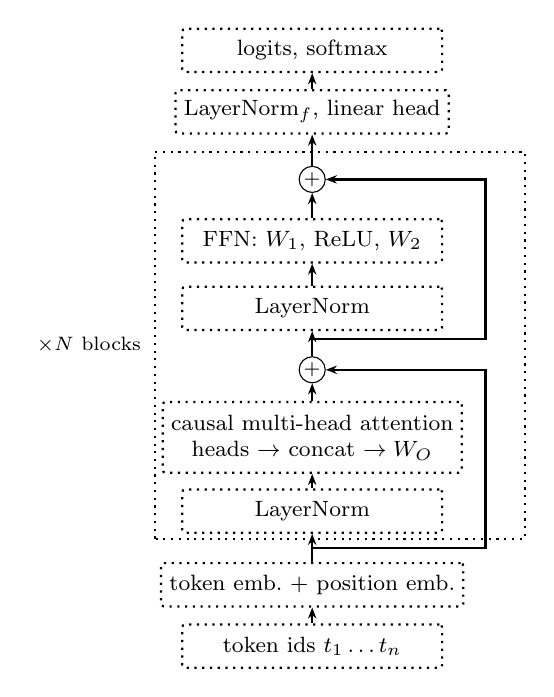
\begin{tikzpicture}[x=1cm,y=0.78cm,every node/.style={font=\scriptsize}]
  \def\w{3.3cm}
  \node[design,minimum width=\w,minimum height=0.55cm] (in) at (0,0) {token ids $t_1\dots t_n$};
  \node[design,minimum width=\w,minimum height=0.55cm] (emb) at (0,1) {token emb.\ $+$ position emb.};
  \node[design,minimum width=\w,minimum height=0.55cm] (ln1) at (0,2.2) {LayerNorm};
  \node[design,minimum width=\w,minimum height=0.9cm,align=center] (mha) at (0,3.4) {causal multi-head attention\\heads $\to$ concat $\to W_O$};
  \node[draw,circle,inner sep=0.5pt] (add1) at (0,4.5) {$+$};
  \node[design,minimum width=\w,minimum height=0.55cm] (ln2) at (0,5.5) {LayerNorm};
  \node[design,minimum width=\w,minimum height=0.55cm] (ff) at (0,6.6) {FFN: $W_1$, ReLU, $W_2$};
  \node[draw,circle,inner sep=0.5pt] (add2) at (0,7.6) {$+$};
  \node[design,minimum width=\w,minimum height=0.55cm] (lnf) at (0,8.7) {LayerNorm$_f$, linear head};
  \node[design,minimum width=\w,minimum height=0.55cm] (out) at (0,9.7) {logits, softmax};
  \draw[arr] (in)--(emb); \draw[arr] (emb)--(ln1); \draw[arr] (ln1)--(mha); \draw[arr] (mha)--(add1);
  \draw[arr] (add1)--(ln2); \draw[arr] (ln2)--(ff); \draw[arr] (ff)--(add2); \draw[arr] (add2)--(lnf); \draw[arr] (lnf)--(out);
  \draw[arr] (0,1.6) -- (2.2,1.6) |- (add1.east);
  \draw[arr] (0,5.0) -- (2.2,5.0) |- (add2.east);
  \draw[thick,dotted] (-2.0,1.75) rectangle (2.7,8.05);
  \node[anchor=east] at (-2.05,4.9) {$\times N$ blocks};
\end{tikzpicture}
\caption{Designed decoder-only block (pre-LN), after the study note's steps 3--5~\cite{note} and Vaswani et al.~\cite{vaswani2017}. Attention is $\mathrm{softmax}(QK^{\top}/\sqrt{d_k}+M)V$ per head, Eq.~\eqref{eq:attn}. Dotted: specified, not trained.}
\label{fig:arch}
\end{figure}

\textbf{Equations (added; the note has none).} With $X$ the sequence of embeddings,
\begin{align}
Q&=XW_Q+b_Q,\; K=XW_K+b_K,\; V=XW_V+b_V \label{eq:qkv}\\
\mathrm{Attn}(X)&=\mathrm{softmax}\!\Big(\tfrac{QK^{\top}}{\sqrt{d_k}}+M\Big)V,\; M_{ij}=-\infty\ (j>i) \label{eq:attn}\\
\mathcal L(\theta)&=-\tfrac1n\textstyle\sum_{i}\log p_\theta(t_{i+1}\mid t_{\le i}) \label{eq:ce}
\end{align}
For $D=32$ and $F=128$, a pre-LN block has $4(D^2{+}D)+2(2D)+(DF{+}F)+(FD{+}D)=\blockParamsSmall$ parameters (analytic count from the block definition; not read from a trained model).

%% ------------------------------------------------------------------------
\section{The Reasoning Gap}\label{sec:gap}
We separate what is measured from what is argued.

\textbf{Measured.} (a)~Different seeds give different weights for the same function (Table~\ref{tab:xor}, Fig.~\ref{fig:geometry}). (b)~A fitted model can return a wrong answer with a high score (Sec.~\ref{sec:measured}).

\textbf{By construction.} Eq.~\eqref{eq:ce} depends on the predicted distribution only; it contains no term for evidence, rule or justification. A model that minimises it can be right for the wrong reason, and nothing in training detects this. This is a property of the objective, not an experimental finding.

\textbf{Not shown.} We have no reasoning benchmark and no trained transformer, so we do not claim that attention models \emph{fail} at reasoning, nor how a small model compares with a large one. Our corpus is tiny; it demonstrates the mechanism, not scale behaviour. Stability of the function across seeds (Sec.~\ref{sec:measured}) is evidence \emph{against} a strong reading of ``random'' and is reported as such.

%% ------------------------------------------------------------------------
\section{Neuro-Symbolic Design (Not Implemented)}\label{sec:ns}
\subsection{Taxonomy mapping}
Fig.~\ref{fig:taxonomy} redraws Fig.~1 of~\cite{sheth2023}, including its low/medium/high ratings, and marks where each proposed component sits. A logit mask or bias is a \emph{lowering}-style intervention only by analogy: \cite{sheth2023} compresses knowledge into embeddings or logic representations, while we apply it to the output scores. A verifier with a trace is a decoupled \emph{lifting} method (2a). A training-time semantic loss~\cite{xu2018} would move toward 2b and is future work.

\begin{figure*}[t]
\centering
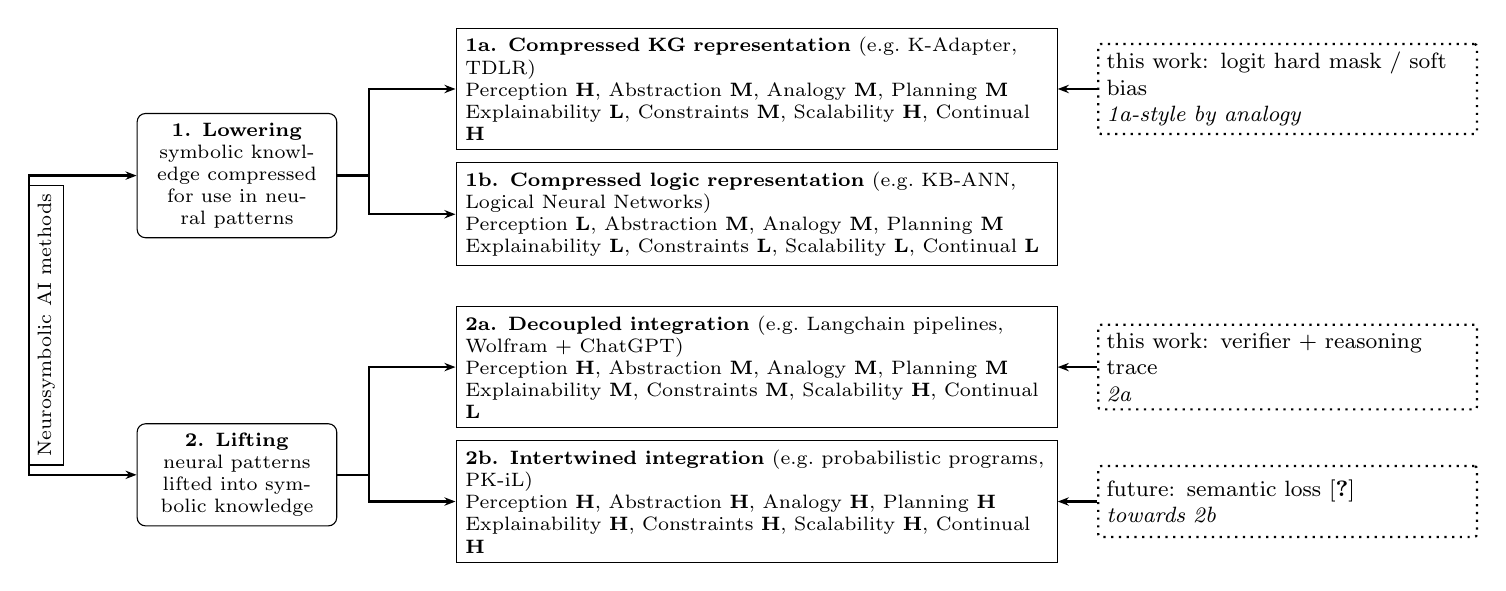
\begin{tikzpicture}[x=1cm,y=1cm,font=\scriptsize]
  \node[draw,rotate=90,anchor=south,inner sep=3pt] (root) at (-0.2,2.5) {Neurosymbolic AI methods};
  \node[draw,rounded corners=3pt,align=center,text width=2.3cm] (c1) at (2.0,4.4) {\textbf{1. Lowering}\\symbolic knowledge compressed for use in neural patterns};
  \node[draw,rounded corners=3pt,align=center,text width=2.3cm] (c2) at (2.0,0.6) {\textbf{2. Lifting}\\neural patterns lifted into symbolic knowledge};
  \draw[arr] (root.north) |- (c1.west); \draw[arr] (root.north) |- (c2.west);
  % rows
  \def\row#1#2#3#4#5#6#7#8#9{}
  \node[draw,align=left,text width=7.4cm] (r1a) at (8.6,5.5) {\textbf{1a. Compressed KG representation} (e.g.\ K-Adapter, TDLR)\\ Perception \textbf{H}, Abstraction \textbf{M}, Analogy \textbf{M}, Planning \textbf{M}\\ Explainability \textbf{L}, Constraints \textbf{M}, Scalability \textbf{H}, Continual \textbf{H}};
  \node[draw,align=left,text width=7.4cm,below=0.15cm of r1a] (r1b) {\textbf{1b. Compressed logic representation} (e.g.\ KB-ANN, Logical Neural Networks)\\ Perception \textbf{L}, Abstraction \textbf{M}, Analogy \textbf{M}, Planning \textbf{M}\\ Explainability \textbf{L}, Constraints \textbf{L}, Scalability \textbf{L}, Continual \textbf{L}};
  \node[draw,align=left,text width=7.4cm,below=0.5cm of r1b] (r2a) {\textbf{2a. Decoupled integration} (e.g.\ Langchain pipelines, Wolfram + ChatGPT)\\ Perception \textbf{H}, Abstraction \textbf{M}, Analogy \textbf{M}, Planning \textbf{M}\\ Explainability \textbf{M}, Constraints \textbf{M}, Scalability \textbf{H}, Continual \textbf{L}};
  \node[draw,align=left,text width=7.4cm,below=0.15cm of r2a] (r2b) {\textbf{2b. Intertwined integration} (e.g.\ probabilistic programs, PK-iL)\\ Perception \textbf{H}, Abstraction \textbf{H}, Analogy \textbf{H}, Planning \textbf{H}\\ Explainability \textbf{H}, Constraints \textbf{H}, Scalability \textbf{H}, Continual \textbf{H}};
  \draw[arr] (c1.east) -- ++(0.4,0) |- (r1a.west); \draw[arr] (c1.east) -- ++(0.4,0) |- (r1b.west);
  \draw[arr] (c2.east) -- ++(0.4,0) |- (r2a.west); \draw[arr] (c2.east) -- ++(0.4,0) |- (r2b.west);
  % our mapping
  \node[design,align=left,text width=4.6cm,right=0.5cm of r1a] (m1) {this work: logit hard mask / soft bias\\\emph{1a-style by analogy}};
  \node[design,align=left,text width=4.6cm,right=0.5cm of r2a] (m2) {this work: verifier + reasoning trace\\\emph{2a}};
  \node[design,align=left,text width=4.6cm,right=0.5cm of r2b] (m3) {future: semantic loss~\cite{xu2018}\\\emph{towards 2b}};
  \draw[arr] (m1) -- (r1a); \draw[arr] (m2) -- (r2a); \draw[arr] (m3) -- (r2b);
\end{tikzpicture}
\caption{Taxonomy of~\cite{sheth2023} (redrawn from its Fig.~1; L/M/H = low/medium/high as rated by those authors) with the position of each component in this work. Dotted boxes are our mapping, not the original authors'.}
\label{fig:taxonomy}
\end{figure*}

\subsection{Mechanisms and the code seam}
Fig.~\ref{fig:ns} shows the intended data flow. A knowledge base of triples and Horn-style rules is expanded by forward chaining. A \emph{logits processor} receives a fresh copy of the length-$V$ logit vector before temperature and softmax: banned tokens are set to $-\infty$ (which stays $-\infty$ after temperature and top-$p$), supported tokens receive $+\lambda$, and if every token would be banned the processor falls back to the unmasked logits and records that in the trace. Each step logs $\{$rules fired, masked tokens, probability mass before and after, chosen token$\}$. A decoupled verifier checks the final text against the same knowledge base.

\begin{figure}[t]
\centering
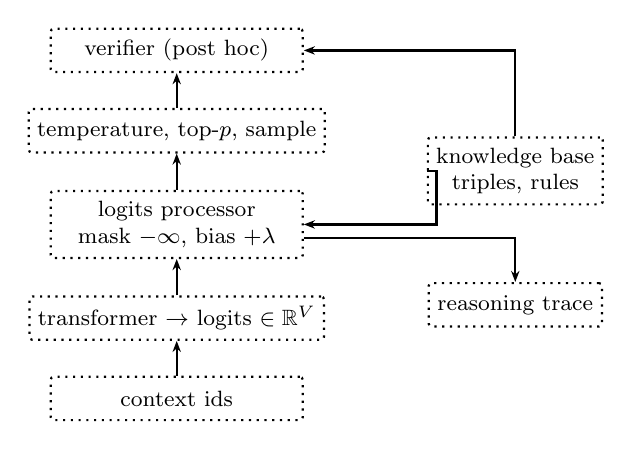
\begin{tikzpicture}[x=1cm,y=0.85cm,every node/.style={font=\scriptsize}]
  \node[design,minimum width=3.2cm,minimum height=0.55cm] (ctx) at (0,0) {context ids};
  \node[design,minimum width=3.2cm,minimum height=0.55cm] (tr) at (0,1.2) {transformer $\to$ logits $\in\mathbb R^V$};
  \node[design,minimum width=3.2cm,minimum height=0.85cm,align=center] (lp) at (0,2.6) {logits processor\\mask $-\infty$, bias $+\lambda$};
  \node[design,minimum width=3.2cm,minimum height=0.55cm] (sm) at (0,4.0) {temperature, top-$p$, sample};
  \node[design,minimum width=3.2cm,minimum height=0.55cm] (v) at (0,5.2) {verifier (post hoc)};
  \node[design,minimum width=2.2cm,minimum height=0.85cm,align=center] (kb) at (4.3,3.4) {knowledge base\\triples, rules};
  \node[design,minimum width=2.2cm,minimum height=0.55cm] (trace) at (4.3,1.4) {reasoning trace};
  \draw[arr] (ctx)--(tr); \draw[arr] (tr)--(lp); \draw[arr] (lp)--(sm); \draw[arr] (sm)--(v);
  \draw[arr] (kb.west) -- (3.3,3.4) |- (lp.east);
  \draw[arr] (kb.north) |- (v.east);
  \draw[arr] (lp.east) ++(0,-0.2) -| (trace.north);
\end{tikzpicture}
\caption{Proposed neuro-symbolic data flow. Nothing in this figure is implemented.}
\label{fig:ns}
\end{figure}

\subsection{Falsifiable predictions and protocol}
Experiments are \emph{specified}, not run. \textbf{E1} (seed sensitivity): train the transformer under four seeds; report final loss spread and weight-space distance. \textbf{E2} (constraint violations): generate $N$ samples per seed with the processor off and on; report KB-violation rate, perplexity and distinct-token ratio. \textbf{E3}: one generation with its full trace. Predictions that would be \emph{refuted} by a bad result: P1, with the hard mask on the violation rate for token-expressible constraints is $0$; P2, with the processor off, generation is byte-identical to the unconstrained baseline for the same seed; P3, loss spread across seeds is small while weight distance is large; P4, a soft bias lowers violations without eliminating them. P1--P2 are properties of the design and can fail only through bugs; P3--P4 are empirical.

%% ------------------------------------------------------------------------
\section{Threats to Validity and Limitations}\label{sec:threats}
\begin{itemize}
\item \emph{Scale.} $\sgSent$ sentences and $\sgVocab$ words. Results demonstrate mechanisms, not scale behaviour.
\item \emph{Few seeds, no tests.} Four seeds per configuration, no confidence intervals or significance tests; ranges are reported as observed.
\item \emph{Answer key.} The analogy key is one answer per query chosen by us; alternative acceptable answers would change the accuracy column.
\item \emph{No held-out evaluation.} Skip-gram is judged on the training corpus; XOR has four points by definition.
\item \emph{Single configuration.} One dimensionality, window and learning rate. No ablation.
\item \emph{Symbolic constraints act on tokens.} Words split into several subword tokens can be constrained only on their first token.
\item \emph{Saved artefact.} The tracked \texttt{.data/embedding-weights.json} still holds the earlier, collapsed model; the numbers here come from fresh runs with saving off.
\end{itemize}

%% ------------------------------------------------------------------------
\section{Conclusion and Future Work}
Stages 0--3 are repaired and measured. Their seeds agree on function and disagree on weights, which supports a refined form of the note's observation. The hypothesis that fitted weights lack justification is, in Eq.~\eqref{eq:ce}, true by construction, and the wrong-but-confident analogy illustrates it; whether a symbolic layer closes the gap is untested. The next steps, in order, are to finish the transformer (forward, backward, Adam) with finite-difference gradient checks; implement the logits processor and verifier; run E1--E3; and replace this paper's ``not implemented'' statements with measured results.

\section*{Provenance}
Fig.~\ref{fig:taxonomy} is redrawn from~\cite{sheth2023}; Fig.~\ref{fig:arch} follows the study note~\cite{note}. No figure is a copy of a published figure, and no code from the reference repository~\cite{howllms} was copied.

\begin{thebibliography}{99}
\bibitem{note} N.~Pham, ``NLP Transformer Note,'' unpublished study note, 5~pp., 2026 (\texttt{docs/paper/}).
\bibitem{sheth2023} A.~Sheth, K.~Roy, and M.~Gaur, ``Neurosymbolic artificial intelligence (why, what, and how),'' \emph{IEEE Intell. Syst.}, vol.~38, no.~3, pp.~56--62, May/Jun. 2023.
\bibitem{vaswani2017} A.~Vaswani \emph{et al.}, ``Attention is all you need,'' in \emph{Proc. NeurIPS}, 2017.
\bibitem{ba2016} J.~L.~Ba, J.~R.~Kiros, and G.~E.~Hinton, ``Layer normalization,'' arXiv:1607.06450, 2016.
\bibitem{kingma2015} D.~P.~Kingma and J.~Ba, ``Adam: A method for stochastic optimization,'' in \emph{Proc. ICLR}, 2015.
\bibitem{weizenbaum1966} J.~Weizenbaum, ``ELIZA---a computer program for the study of natural language communication between man and machine,'' \emph{Commun. ACM}, vol.~9, no.~1, pp.~36--45, 1966.
\bibitem{sennrich2016} R.~Sennrich, B.~Haddow, and A.~Birch, ``Neural machine translation of rare words with subword units,'' in \emph{Proc. ACL}, 2016, pp.~1715--1725.
\bibitem{rumelhart1986} D.~E.~Rumelhart, G.~E.~Hinton, and R.~J.~Williams, ``Learning representations by back-propagating errors,'' \emph{Nature}, vol.~323, pp.~533--536, 1986.
\bibitem{mikolov2013a} T.~Mikolov, K.~Chen, G.~Corrado, and J.~Dean, ``Efficient estimation of word representations in vector space,'' arXiv:1301.3781, 2013.
\bibitem{mikolov2013b} T.~Mikolov, I.~Sutskever, K.~Chen, G.~Corrado, and J.~Dean, ``Distributed representations of words and phrases and their compositionality,'' in \emph{Proc. NeurIPS}, 2013.
\bibitem{xu2018} J.~Xu, Z.~Zhang, T.~Friedman, Y.~Liang, and G.~Van den Broeck, ``A semantic loss function for deep learning with symbolic knowledge,'' in \emph{Proc. ICML}, 2018.
\bibitem{howllms} w3cj, ``how-llms-work,'' GitHub repository, \url{https://github.com/w3cj/how-llms-work} (no licence file; architecture cross-check only).
\end{thebibliography}
\end{document}
